	
\begin{figure}


	\centering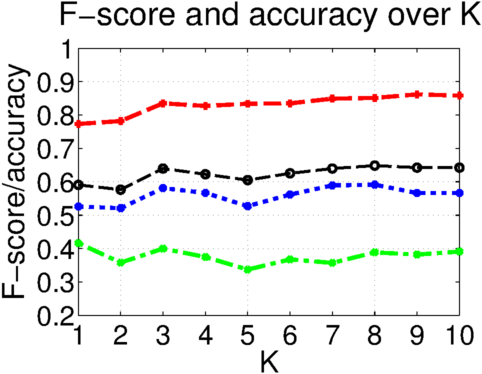
\includegraphics[width=0.3\textwidth]{tex/appendices/test/sskew2010FP.png}
	\centering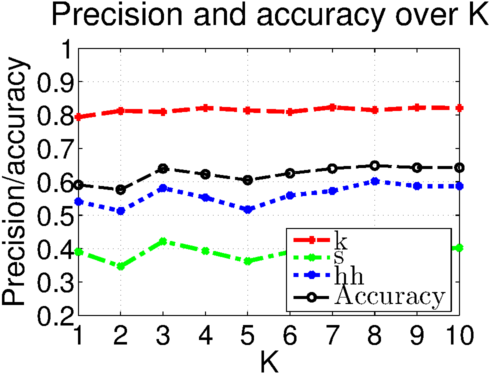
\includegraphics[width=0.3\textwidth]{tex/appendices/test/sskew2010_P.png}	g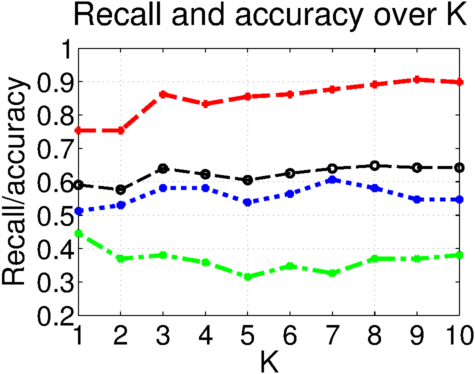
\includegraphics[width=0.3\textwidth]{tex/appendices/test/sskew2010_R.png}
	
	\caption{Plots over K for Spectral Skew with 20ms windows and 10ms window skips}
\end{figure}

\begin{figure}

	\centering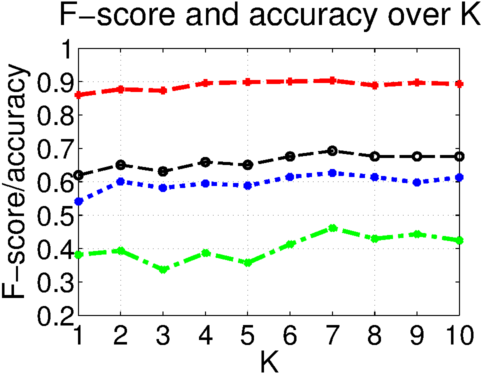
\includegraphics[width=0.3\textwidth]{tex/appendices/test/sskew105FP.png}
	\centering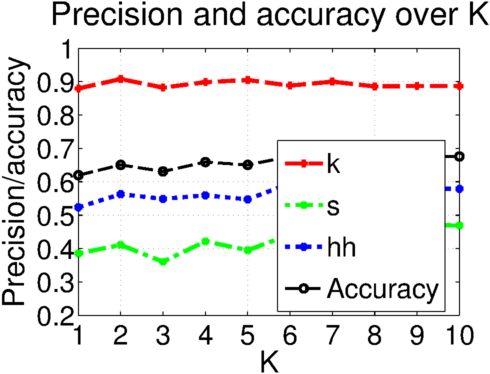
\includegraphics[width=0.3\textwidth]{tex/appendices/test/sskew105_P.png}
	\centering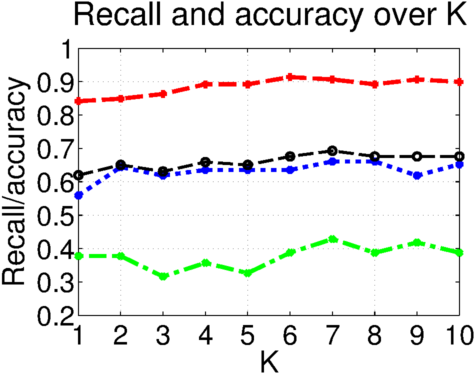
\includegraphics[width=0.3\textwidth]{tex/appendices/test/sskew105_R.png}
		
		\caption{Plots over K for Spectral Skew with 10ms windows and 5ms window skips}
\label{figJitter}
\end{figure}
\begin{figure}


	\centering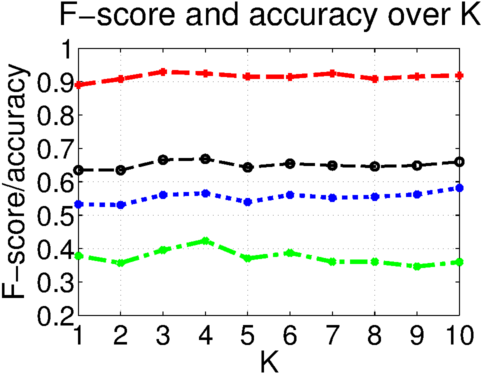
\includegraphics[width=0.3\textwidth]{tex/appendices/test/sskew52FP.png}
	\centering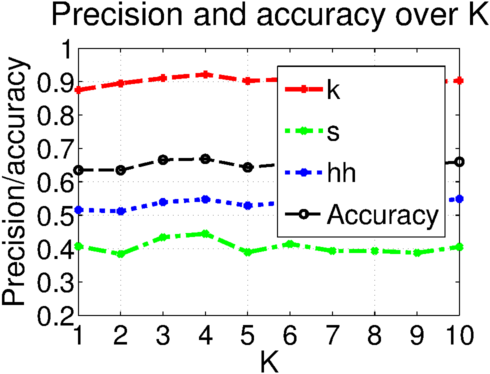
\includegraphics[width=0.3\textwidth]{tex/appendices/test/sskew52_P.png}
	\centering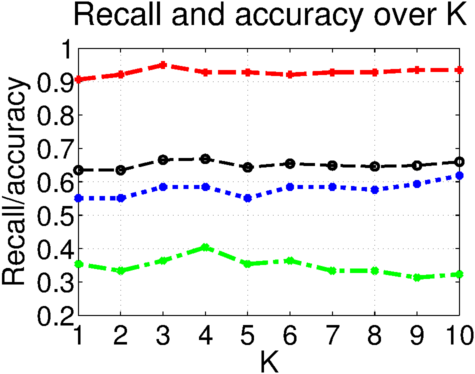
\includegraphics[width=0.3\textwidth]{tex/appendices/test/sskew52_R.png}
		
		\caption{Plots over K for Spectral Skew with 5ms windows and 2ms window skips}
\end{figure}\clearpage



\begin{table}
\begin{subtable}[tbp]{0.45\textwidth}
\centering
\begin{tabular}{|c|c|c|c"c|}
\cline{2-5}
 \multicolumn{1}{c|}{} & \textbf{k}  & \textbf{s}  & \textbf{hh}  & Prec.\\ \hline
 \textbf{k} & \textcolor{red}{0.754} & 0.152 & 0.111 & 0.794\\ \hline
 \textbf{s} & 0.145 & \textcolor{red}{0.446} & 0.376 & 0.390\\ \hline
 \textbf{hh} & 0.145 & 0.402 & \textcolor{red}{0.513} & 0.541\\ \Xhline{2\arrayrulewidth}
 F & 0.773 & 0.416 & 0.526 & \textcolor{blue}{0.591}\\ \hline
\end{tabular}
\caption{$K=1$}
\end{subtable}
\hfill
\begin{subtable}[tbp]{0.45\textwidth}
\centering
\begin{tabular}{|c|c|c|c"c|}
\cline{2-5}
 \multicolumn{1}{c|}{} & \textbf{k}  & \textbf{s}  & \textbf{hh}  & Prec.\\ \hline
 \textbf{k} & \textcolor{red}{0.754} & 0.152 & 0.085 & 0.812\\ \hline
 \textbf{s} & 0.138 & \textcolor{red}{0.370} & 0.385 & 0.347\\ \hline
 \textbf{hh} & 0.138 & 0.478 & \textcolor{red}{0.530} & 0.512\\ \Xhline{2\arrayrulewidth}
 F & 0.782 & 0.358 & 0.521 & \textcolor{blue}{0.576}\\ \hline
\end{tabular}
\caption{$K=2$}
\label{app:SS:2:worst}
\end{subtable}
\hfill
\begin{subtable}[tbp]{0.45\textwidth}
\centering
\begin{tabular}{|c|c|c|c"c|}
\cline{2-5}
 \multicolumn{1}{c|}{} & \textbf{k}  & \textbf{s}  & \textbf{hh}  & Prec.\\ \hline
 \textbf{k} & \textcolor{red}{0.862} & 0.185 & 0.094 & 0.810\\ \hline
 \textbf{s} & 0.072 & \textcolor{red}{0.380} & 0.325 & 0.422\\ \hline
 \textbf{hh} & 0.072 & 0.435 & \textcolor{red}{0.581} & 0.581\\ \Xhline{2\arrayrulewidth}
 F & 0.835 & 0.400 & 0.581 & \textcolor{blue}{0.640}\\ \hline
\end{tabular}
\caption{$K=3$}
\end{subtable}
\hfill
\begin{subtable}[tbp]{0.45\textwidth}
\centering
\begin{tabular}{|c|c|c|c"c|}
\cline{2-5}
 \multicolumn{1}{c|}{} & \textbf{k}  & \textbf{s}  & \textbf{hh}  & Prec.\\ \hline
 \textbf{k} & \textcolor{red}{0.833} & 0.152 & 0.094 & 0.821\\ \hline
 \textbf{s} & 0.094 & \textcolor{red}{0.359} & 0.325 & 0.393\\ \hline
 \textbf{hh} & 0.094 & 0.489 & \textcolor{red}{0.581} & 0.553\\ \Xhline{2\arrayrulewidth}
 F & 0.827 & 0.375 & 0.567 & \textcolor{blue}{0.622}\\ \hline
\end{tabular}
\caption{$K=4$}
\end{subtable}
\hfill
\begin{subtable}[tbp]{0.45\textwidth}
\centering
\begin{tabular}{|c|c|c|c"c|}
\cline{2-5}
 \multicolumn{1}{c|}{} & \textbf{k}  & \textbf{s}  & \textbf{hh}  & Prec.\\ \hline
 \textbf{k} & \textcolor{red}{0.855} & 0.152 & 0.111 & 0.814\\ \hline
 \textbf{s} & 0.072 & \textcolor{red}{0.315} & 0.350 & 0.362\\ \hline
 \textbf{hh} & 0.072 & 0.533 & \textcolor{red}{0.538} & 0.516\\ \Xhline{2\arrayrulewidth}
 F & 0.834 & 0.337 & 0.527 & \textcolor{blue}{0.605}\\ \hline
\end{tabular}
\caption{$K=5$}
\end{subtable}
\hfill
\begin{subtable}[tbp]{0.45\textwidth}
\centering
\begin{tabular}{|c|c|c|c"c|}
\cline{2-5}
 \multicolumn{1}{c|}{} & \textbf{k}  & \textbf{s}  & \textbf{hh}  & Prec.\\ \hline
 \textbf{k} & \textcolor{red}{0.862} & 0.163 & 0.111 & 0.810\\ \hline
 \textbf{s} & 0.087 & \textcolor{red}{0.348} & 0.325 & 0.390\\ \hline
 \textbf{hh} & 0.087 & 0.489 & \textcolor{red}{0.564} & 0.559\\ \Xhline{2\arrayrulewidth}
 F & 0.835 & 0.368 & 0.562 & \textcolor{blue}{0.625}\\ \hline
\end{tabular}
\caption{$K=6$}
\end{subtable}
\hfill
\begin{subtable}[tbp]{0.45\textwidth}
\centering
\begin{tabular}{|c|c|c|c"c|}
\cline{2-5}
 \multicolumn{1}{c|}{} & \textbf{k}  & \textbf{s}  & \textbf{hh}  & Prec.\\ \hline
 \textbf{k} & \textcolor{red}{0.877} & 0.163 & 0.094 & 0.823\\ \hline
 \textbf{s} & 0.080 & \textcolor{red}{0.326} & 0.299 & 0.395\\ \hline
 \textbf{hh} & 0.080 & 0.511 & \textcolor{red}{0.607} & 0.573\\ \Xhline{2\arrayrulewidth}
 F & 0.849 & 0.357 & 0.589 & \textcolor{blue}{0.640}\\ \hline
\end{tabular}
\caption{$K=7$}
\end{subtable}
\hfill
\begin{subtable}[tbp]{0.45\textwidth}
\centering
\begin{tabular}{|c|c|c|c"c|}
\cline{2-5}
 \multicolumn{1}{c|}{} & \textbf{k}  & \textbf{s}  & \textbf{hh}  & Prec.\\ \hline
 \textbf{k} & \textcolor{red}{0.891} & 0.174 & 0.103 & 0.815\\ \hline
 \textbf{s} & 0.087 & \textcolor{red}{0.370} & 0.316 & 0.410\\ \hline
 \textbf{hh} & 0.087 & 0.457 & \textcolor{red}{0.581} & 0.602\\ \Xhline{2\arrayrulewidth}
 F & 0.851 & 0.389 & 0.591 & \textcolor{blue}{0.648}\\ \hline
\end{tabular}
\caption{$K=8$}
\end{subtable}
\hfill
\begin{subtable}[tbp]{0.45\textwidth}
\centering
\begin{tabular}{|c|c|c|c"c|}
\cline{2-5}
 \multicolumn{1}{c|}{} & \textbf{k}  & \textbf{s}  & \textbf{hh}  & Prec.\\ \hline
 \textbf{k} & \textcolor{red}{0.906} & 0.163 & 0.103 & 0.822\\ \hline
 \textbf{s} & 0.080 & \textcolor{red}{0.370} & 0.350 & 0.395\\ \hline
 \textbf{hh} & 0.080 & 0.467 & \textcolor{red}{0.547} & 0.587\\ \Xhline{2\arrayrulewidth}
 F & 0.862 & 0.382 & 0.566 & \textcolor{blue}{0.643}\\ \hline
\end{tabular}
\caption{$K=9$}
\end{subtable}
\hfill
\begin{subtable}[tbp]{0.45\textwidth}
\centering
\begin{tabular}{|c|c|c|c"c|}
\cline{2-5}
 \multicolumn{1}{c|}{} & \textbf{k}  & \textbf{s}  & \textbf{hh}  & Prec.\\ \hline
 \textbf{k} & \textcolor{red}{0.899} & 0.163 & 0.103 & 0.821\\ \hline
 \textbf{s} & 0.080 & \textcolor{red}{0.380} & 0.350 & 0.402\\ \hline
 \textbf{hh} & 0.080 & 0.457 & \textcolor{red}{0.547} & 0.587\\ \Xhline{2\arrayrulewidth}
 F & 0.858 & 0.391 & 0.566 & \textcolor{blue}{0.643}\\ \hline
\end{tabular}
\caption{$K=10$}
\end{subtable}
\hfill


\caption{tcsskew2010}
\label{tlsskew2010}

\end{table}\clearpage


\begin{table}

\begin{subtable}[tbp]{0.45\textwidth}
\centering

\scalebox{0.8}{\begin{tabular}{|c|c|c|c|}\hline
 $K_1$ & $K_2$ & $X^2$ & p\\ \hline
 1 & 2 & 63.000 & 0.24255\\ \hline 
 1 & 3 & 63.000 & 0.24255\\ \hline 
 1 & 4 & 63.000 & 0.24255\\ \hline 
 1 & 5 & 56.250 & 0.22185\\ \hline 
 1 & 6 & 63.000 & 0.24255\\ \hline 
 1 & 7 & 54.000 & 0.28935\\ \hline 
 1 & 8 & 54.000 & 0.28935\\ \hline 
 1 & 9 & 63.000 & 0.24255\\ \hline 
 1 & 10 & 63.000 & 0.24255\\ \hline 
 2 & 3 & 72.000 & 0.23040\\ \hline 
 2 & 4 & 72.000 & 0.23040\\ \hline 
 2 & 5 & 63.000 & 0.24255\\ \hline 
 2 & 6 & 72.000 & 0.23040\\ \hline 
 2 & 7 & 63.000 & 0.24255\\ \hline 
 2 & 8 & 63.000 & 0.24255\\ \hline 
 2 & 9 & 72.000 & 0.23040\\ \hline 
 2 & 10 & 72.000 & 0.23040\\ \hline 
 3 & 4 & 72.000 & 0.23040\\ \hline 
 3 & 5 & 63.000 & 0.24255\\ \hline 
 3 & 6 & 72.000 & 0.23040\\ \hline 
 3 & 7 & 63.000 & 0.24255\\ \hline 
 3 & 8 & 63.000 & 0.24255\\ \hline 
 3 & 9 & 72.000 & 0.23040\\ \hline 
 3 & 10 & 72.000 & 0.23040\\ \hline 
 4 & 5 & 63.000 & 0.24255\\ \hline 
 4 & 6 & 72.000 & 0.23040\\ \hline 
 4 & 7 & 63.000 & 0.24255\\ \hline 
 4 & 8 & 63.000 & 0.24255\\ \hline 
 4 & 9 & 72.000 & 0.23040\\ \hline 
 4 & 10 & 72.000 & 0.23040\\ \hline 
 5 & 6 & 63.000 & 0.24255\\ \hline 
 5 & 7 & 56.250 & 0.22185\\ \hline 
 5 & 8 & 56.250 & 0.22185\\ \hline 
 5 & 9 & 63.000 & 0.24255\\ \hline 
 5 & 10 & 63.000 & 0.24255\\ \hline 
 6 & 7 & 63.000 & 0.24255\\ \hline 
 6 & 8 & 63.000 & 0.24255\\ \hline 
 6 & 9 & 72.000 & 0.23040\\ \hline 
 6 & 10 & 72.000 & 0.23040\\ \hline 
 7 & 8 & 63.000 & 0.08640\\ \hline 
 7 & 9 & 63.000 & 0.24255\\ \hline 
 7 & 10 & 63.000 & 0.24255\\ \hline 
 8 & 9 & 63.000 & 0.24255\\ \hline 
 8 & 10 & 63.000 & 0.24255\\ \hline 
 9 & 10 & 72.000 & 0.23040\\ \hline 

\end{tabular}
}\caption{xcsskew2010} \label{xlsskew2010}

\end{subtable}

\begin{subtable}[tbp]{0.45\textwidth}
\centering
\begin{tabular}{|c|c|c|}
\hline
Class & Amount & Percent\\ \hline
k & 461 & 32.93\\ \hline
undefined & 125 & 8.93\\ \hline
s & 307 & 21.93\\ \hline
\end{tabular}
\caption{Entire dataset after stripping short sounds}
\end{subtable}
\hfill
\begin{subtable}[tbp]{0.45\textwidth}
\centering
\begin{tabular}{|c|c|c|}
\hline
Class & Amount & Percent\\ \hline
k & 322 & 39.80\\ \hline
s & 214 & 26.45\\ \hline
hh & 273 & 33.75\\ \hline
\end{tabular}
\caption{Training dataset}
\end{subtable}
\hfill
\begin{subtable}[tbp]{0.45\textwidth}
\centering
\begin{tabular}{|c|c|c|}
\hline
Class & Amount & Percent\\ \hline
k & 138 & 39.77\\ \hline
s & 92 & 26.51\\ \hline
hh & 117 & 33.72\\ \hline
\end{tabular}
\caption{Testing dataset}
\end{subtable}
\hfill

\label{dlsskew2010}
\caption{dcsskew2010}


\end{table}\clearpage


\begin{table}
\begin{subtable}[tbp]{0.45\textwidth}
\centering
\begin{tabular}{|c|c|c|c"c|}
\cline{2-5}
 \multicolumn{1}{c|}{} & \textbf{k}  & \textbf{s}  & \textbf{hh}  & Prec.\\ \hline
 \textbf{k} & \textcolor{red}{0.842} & 0.122 & 0.034 & 0.880\\ \hline
 \textbf{s} & 0.079 & \textcolor{red}{0.378} & 0.407 & 0.385\\ \hline
 \textbf{hh} & 0.079 & 0.500 & \textcolor{red}{0.559} & 0.524\\ \Xhline{2\arrayrulewidth}
 F & 0.860 & 0.381 & 0.541 & \textcolor{blue}{0.620}\\ \hline
\end{tabular}
\caption{$K=1$}
\end{subtable}
\hfill
\begin{subtable}[tbp]{0.45\textwidth}
\centering
\begin{tabular}{|c|c|c|c"c|}
\cline{2-5}
 \multicolumn{1}{c|}{} & \textbf{k}  & \textbf{s}  & \textbf{hh}  & Prec.\\ \hline
 \textbf{k} & \textcolor{red}{0.849} & 0.092 & 0.025 & 0.908\\ \hline
 \textbf{s} & 0.101 & \textcolor{red}{0.378} & 0.331 & 0.411\\ \hline
 \textbf{hh} & 0.101 & 0.531 & \textcolor{red}{0.644} & 0.563\\ \Xhline{2\arrayrulewidth}
 F & 0.877 & 0.394 & 0.601 & \textcolor{blue}{0.651}\\ \hline
\end{tabular}
\caption{$K=2$}
\end{subtable}
\hfill
\begin{subtable}[tbp]{0.45\textwidth}
\centering
\begin{tabular}{|c|c|c|c"c|}
\cline{2-5}
 \multicolumn{1}{c|}{} & \textbf{k}  & \textbf{s}  & \textbf{hh}  & Prec.\\ \hline
 \textbf{k} & \textcolor{red}{0.863} & 0.133 & 0.025 & 0.882\\ \hline
 \textbf{s} & 0.094 & \textcolor{red}{0.316} & 0.356 & 0.360\\ \hline
 \textbf{hh} & 0.094 & 0.551 & \textcolor{red}{0.619} & 0.549\\ \Xhline{2\arrayrulewidth}
 F & 0.873 & 0.337 & 0.582 & \textcolor{blue}{0.631}\\ \hline
\end{tabular}
\caption{$K=3$}
\end{subtable}
\hfill
\begin{subtable}[tbp]{0.45\textwidth}
\centering
\begin{tabular}{|c|c|c|c"c|}
\cline{2-5}
 \multicolumn{1}{c|}{} & \textbf{k}  & \textbf{s}  & \textbf{hh}  & Prec.\\ \hline
 \textbf{k} & \textcolor{red}{0.892} & 0.102 & 0.034 & 0.899\\ \hline
 \textbf{s} & 0.065 & \textcolor{red}{0.357} & 0.331 & 0.422\\ \hline
 \textbf{hh} & 0.065 & 0.541 & \textcolor{red}{0.636} & 0.560\\ \Xhline{2\arrayrulewidth}
 F & 0.895 & 0.387 & 0.595 & \textcolor{blue}{0.659}\\ \hline
\end{tabular}
\caption{$K=4$}
\end{subtable}
\hfill
\begin{subtable}[tbp]{0.45\textwidth}
\centering
\begin{tabular}{|c|c|c|c"c|}
\cline{2-5}
 \multicolumn{1}{c|}{} & \textbf{k}  & \textbf{s}  & \textbf{hh}  & Prec.\\ \hline
 \textbf{k} & \textcolor{red}{0.892} & 0.092 & 0.034 & 0.905\\ \hline
 \textbf{s} & 0.072 & \textcolor{red}{0.327} & 0.331 & 0.395\\ \hline
 \textbf{hh} & 0.072 & 0.582 & \textcolor{red}{0.636} & 0.547\\ \Xhline{2\arrayrulewidth}
 F & 0.899 & 0.358 & 0.588 & \textcolor{blue}{0.651}\\ \hline
\end{tabular}
\caption{$K=5$}
\end{subtable}
\hfill
\begin{subtable}[tbp]{0.45\textwidth}
\centering
\begin{tabular}{|c|c|c|c"c|}
\cline{2-5}
 \multicolumn{1}{c|}{} & \textbf{k}  & \textbf{s}  & \textbf{hh}  & Prec.\\ \hline
 \textbf{k} & \textcolor{red}{0.914} & 0.122 & 0.034 & 0.888\\ \hline
 \textbf{s} & 0.065 & \textcolor{red}{0.388} & 0.331 & 0.442\\ \hline
 \textbf{hh} & 0.065 & 0.490 & \textcolor{red}{0.636} & 0.595\\ \Xhline{2\arrayrulewidth}
 F & 0.901 & 0.413 & 0.615 & \textcolor{blue}{0.676}\\ \hline
\end{tabular}
\caption{$K=6$}
\end{subtable}
\hfill
\begin{subtable}[tbp]{0.45\textwidth}
\centering
\begin{tabular}{|c|c|c|c"c|}
\cline{2-5}
 \multicolumn{1}{c|}{} & \textbf{k}  & \textbf{s}  & \textbf{hh}  & Prec.\\ \hline
 \textbf{k} & \textcolor{red}{0.906} & 0.112 & 0.025 & 0.900\\ \hline
 \textbf{s} & 0.036 & \textcolor{red}{0.429} & 0.314 & 0.500\\ \hline
 \textbf{hh} & 0.036 & 0.459 & \textcolor{red}{0.661} & 0.595\\ \Xhline{2\arrayrulewidth}
 F & 0.903 & 0.462 & 0.627 & \textcolor{blue}{0.693}\\ \hline
\end{tabular}
\caption{$K=7$}
\label{app:SS:7:best}
\end{subtable}
\hfill
\begin{subtable}[tbp]{0.45\textwidth}
\centering
\begin{tabular}{|c|c|c|c"c|}
\cline{2-5}
 \multicolumn{1}{c|}{} & \textbf{k}  & \textbf{s}  & \textbf{hh}  & Prec.\\ \hline
 \textbf{k} & \textcolor{red}{0.892} & 0.122 & 0.034 & 0.886\\ \hline
 \textbf{s} & 0.036 & \textcolor{red}{0.388} & 0.305 & 0.481\\ \hline
 \textbf{hh} & 0.036 & 0.490 & \textcolor{red}{0.661} & 0.574\\ \Xhline{2\arrayrulewidth}
 F & 0.889 & 0.429 & 0.614 & \textcolor{blue}{0.676}\\ \hline
\end{tabular}
\caption{$K=8$}
\end{subtable}
\hfill
\begin{subtable}[tbp]{0.45\textwidth}
\centering
\begin{tabular}{|c|c|c|c"c|}
\cline{2-5}
 \multicolumn{1}{c|}{} & \textbf{k}  & \textbf{s}  & \textbf{hh}  & Prec.\\ \hline
 \textbf{k} & \textcolor{red}{0.906} & 0.112 & 0.042 & 0.887\\ \hline
 \textbf{s} & 0.043 & \textcolor{red}{0.418} & 0.339 & 0.471\\ \hline
 \textbf{hh} & 0.043 & 0.469 & \textcolor{red}{0.619} & 0.579\\ \Xhline{2\arrayrulewidth}
 F & 0.897 & 0.443 & 0.598 & \textcolor{blue}{0.676}\\ \hline
\end{tabular}
\caption{$K=9$}
\end{subtable}
\hfill
\begin{subtable}[tbp]{0.45\textwidth}
\centering
\begin{tabular}{|c|c|c|c"c|}
\cline{2-5}
 \multicolumn{1}{c|}{} & \textbf{k}  & \textbf{s}  & \textbf{hh}  & Prec.\\ \hline
 \textbf{k} & \textcolor{red}{0.899} & 0.112 & 0.042 & 0.887\\ \hline
 \textbf{s} & 0.050 & \textcolor{red}{0.388} & 0.305 & 0.469\\ \hline
 \textbf{hh} & 0.050 & 0.500 & \textcolor{red}{0.653} & 0.579\\ \Xhline{2\arrayrulewidth}
 F & 0.893 & 0.425 & 0.614 & \textcolor{blue}{0.676}\\ \hline
\end{tabular}
\caption{$K=10$}
\end{subtable}
\hfill

\label{tlsskew105}

\caption{tcsskew105}

\end{table}\clearpage


\begin{table}

\begin{subtable}[tbp]{0.45\textwidth}
\centering
 
\scalebox{0.8}{\begin{tabular}{|c|c|c|c|}\hline
 $K_1$ & $K_2$ & $X^2$ & p\\ \hline
 1 & 2 & 63.000 & 0.24255\\ \hline 
 1 & 3 & 56.250 & 0.22185\\ \hline 
 1 & 4 & 63.000 & 0.24255\\ \hline 
 1 & 5 & 63.000 & 0.24255\\ \hline 
 1 & 6 & 63.000 & 0.24255\\ \hline 
 1 & 7 & 63.000 & 0.24255\\ \hline 
 1 & 8 & 63.000 & 0.24255\\ \hline 
 1 & 9 & 63.000 & 0.24255\\ \hline 
 1 & 10 & 63.000 & 0.08640\\ \hline 
 2 & 3 & 63.000 & 0.24255\\ \hline 
 2 & 4 & 72.000 & 0.23040\\ \hline 
 2 & 5 & 72.000 & 0.23040\\ \hline 
 2 & 6 & 72.000 & 0.23040\\ \hline 
 2 & 7 & 72.000 & 0.23040\\ \hline 
 2 & 8 & 72.000 & 0.23040\\ \hline 
 2 & 9 & 72.000 & 0.23040\\ \hline 
 2 & 10 & 63.000 & 0.24255\\ \hline 
 3 & 4 & 63.000 & 0.24255\\ \hline 
 3 & 5 & 63.000 & 0.24255\\ \hline 
 3 & 6 & 63.000 & 0.24255\\ \hline 
 3 & 7 & 63.000 & 0.24255\\ \hline 
 3 & 8 & 63.000 & 0.24255\\ \hline 
 3 & 9 & 63.000 & 0.24255\\ \hline 
 3 & 10 & 56.250 & 0.22185\\ \hline 
 4 & 5 & 72.000 & 0.23040\\ \hline 
 4 & 6 & 72.000 & 0.23040\\ \hline 
 4 & 7 & 72.000 & 0.23040\\ \hline 
 4 & 8 & 72.000 & 0.23040\\ \hline 
 4 & 9 & 72.000 & 0.23040\\ \hline 
 4 & 10 & 63.000 & 0.24255\\ \hline 
 5 & 6 & 72.000 & 0.23040\\ \hline 
 5 & 7 & 72.000 & 0.23040\\ \hline 
 5 & 8 & 72.000 & 0.23040\\ \hline 
 5 & 9 & 72.000 & 0.23040\\ \hline 
 5 & 10 & 63.000 & 0.24255\\ \hline 
 6 & 7 & 72.000 & 0.23040\\ \hline 
 6 & 8 & 72.000 & 0.23040\\ \hline 
 6 & 9 & 72.000 & 0.23040\\ \hline 
 6 & 10 & 63.000 & 0.24255\\ \hline 
 7 & 8 & 72.000 & 0.23040\\ \hline 
 7 & 9 & 72.000 & 0.23040\\ \hline 
 7 & 10 & 63.000 & 0.24255\\ \hline 
 8 & 9 & 72.000 & 0.23040\\ \hline 
 8 & 10 & 63.000 & 0.24255\\ \hline 
 9 & 10 & 63.000 & 0.24255\\ \hline 

\end{tabular}
} \caption{xcsskew105}\label{xlsskew105}

\end{subtable}

\begin{subtable}[tbp]{0.45\textwidth}
\centering
\begin{tabular}{|c|c|c|}
\hline
Class & Amount & Percent\\ \hline
noise & 138 & 9.47\\ \hline
k & 466 & 31.98\\ \hline
undefined & 130 & 8.92\\ \hline
\end{tabular}
\caption{Entire dataset after stripping short sounds}
\end{subtable}
\hfill
\begin{subtable}[tbp]{0.45\textwidth}
\centering
\begin{tabular}{|c|c|c|}
\hline
Class & Amount & Percent\\ \hline
k & 326 & 39.23\\ \hline
s & 229 & 27.56\\ \hline
hh & 276 & 33.21\\ \hline
\end{tabular}
\caption{Training dataset}
\end{subtable}
\hfill
\begin{subtable}[tbp]{0.45\textwidth}
\centering
\begin{tabular}{|c|c|c|}
\hline
Class & Amount & Percent\\ \hline
k & 139 & 39.15\\ \hline
s & 98 & 27.61\\ \hline
hh & 118 & 33.24\\ \hline
\end{tabular}
\caption{Testing dataset}
\end{subtable}
\hfill

\label{dlsskew105}
\caption{dcsskew105}


\end{table}\clearpage


\begin{table}
\begin{subtable}[tbp]{0.45\textwidth}
\centering
\begin{tabular}{|c|c|c|c"c|}
\cline{2-5}
 \multicolumn{1}{c|}{} & \textbf{k}  & \textbf{s}  & \textbf{hh}  & Prec.\\ \hline
 \textbf{k} & \textcolor{red}{0.906} & 0.111 & 0.059 & 0.875\\ \hline
 \textbf{s} & 0.036 & \textcolor{red}{0.354} & 0.390 & 0.407\\ \hline
 \textbf{hh} & 0.036 & 0.535 & \textcolor{red}{0.551} & 0.516\\ \Xhline{2\arrayrulewidth}
 F & 0.890 & 0.378 & 0.533 & \textcolor{blue}{0.635}\\ \hline
\end{tabular}
\caption{$K=1$}
\end{subtable}
\hfill
\begin{subtable}[tbp]{0.45\textwidth}
\centering
\begin{tabular}{|c|c|c|c"c|}
\cline{2-5}
 \multicolumn{1}{c|}{} & \textbf{k}  & \textbf{s}  & \textbf{hh}  & Prec.\\ \hline
 \textbf{k} & \textcolor{red}{0.921} & 0.101 & 0.042 & 0.895\\ \hline
 \textbf{s} & 0.036 & \textcolor{red}{0.333} & 0.407 & 0.384\\ \hline
 \textbf{hh} & 0.036 & 0.566 & \textcolor{red}{0.551} & 0.512\\ \Xhline{2\arrayrulewidth}
 F & 0.908 & 0.357 & 0.531 & \textcolor{blue}{0.635}\\ \hline
\end{tabular}
\caption{$K=2$}
\end{subtable}
\hfill
\begin{subtable}[tbp]{0.45\textwidth}
\centering
\begin{tabular}{|c|c|c|c"c|}
\cline{2-5}
 \multicolumn{1}{c|}{} & \textbf{k}  & \textbf{s}  & \textbf{hh}  & Prec.\\ \hline
 \textbf{k} & \textcolor{red}{0.950} & 0.081 & 0.042 & 0.910\\ \hline
 \textbf{s} & 0.022 & \textcolor{red}{0.364} & 0.373 & 0.434\\ \hline
 \textbf{hh} & 0.022 & 0.556 & \textcolor{red}{0.585} & 0.539\\ \Xhline{2\arrayrulewidth}
 F & 0.930 & 0.396 & 0.561 & \textcolor{blue}{0.666}\\ \hline
\end{tabular}
\caption{$K=3$}
\end{subtable}
\hfill
\begin{subtable}[tbp]{0.45\textwidth}
\centering
\begin{tabular}{|c|c|c|c"c|}
\cline{2-5}
 \multicolumn{1}{c|}{} & \textbf{k}  & \textbf{s}  & \textbf{hh}  & Prec.\\ \hline
 \textbf{k} & \textcolor{red}{0.928} & 0.071 & 0.034 & 0.921\\ \hline
 \textbf{s} & 0.036 & \textcolor{red}{0.404} & 0.381 & 0.444\\ \hline
 \textbf{hh} & 0.036 & 0.525 & \textcolor{red}{0.585} & 0.548\\ \Xhline{2\arrayrulewidth}
 F & 0.925 & 0.423 & 0.566 & \textcolor{blue}{0.669}\\ \hline
\end{tabular}
\caption{$K=4$}
\end{subtable}
\hfill
\begin{subtable}[tbp]{0.45\textwidth}
\centering
\begin{tabular}{|c|c|c|c"c|}
\cline{2-5}
 \multicolumn{1}{c|}{} & \textbf{k}  & \textbf{s}  & \textbf{hh}  & Prec.\\ \hline
 \textbf{k} & \textcolor{red}{0.928} & 0.101 & 0.034 & 0.902\\ \hline
 \textbf{s} & 0.043 & \textcolor{red}{0.354} & 0.415 & 0.389\\ \hline
 \textbf{hh} & 0.043 & 0.545 & \textcolor{red}{0.551} & 0.528\\ \Xhline{2\arrayrulewidth}
 F & 0.915 & 0.370 & 0.539 & \textcolor{blue}{0.643}\\ \hline
\end{tabular}
\caption{$K=5$}
\end{subtable}
\hfill
\begin{subtable}[tbp]{0.45\textwidth}
\centering
\begin{tabular}{|c|c|c|c"c|}
\cline{2-5}
 \multicolumn{1}{c|}{} & \textbf{k}  & \textbf{s}  & \textbf{hh}  & Prec.\\ \hline
 \textbf{k} & \textcolor{red}{0.921} & 0.101 & 0.025 & 0.908\\ \hline
 \textbf{s} & 0.036 & \textcolor{red}{0.364} & 0.390 & 0.414\\ \hline
 \textbf{hh} & 0.036 & 0.535 & \textcolor{red}{0.585} & 0.539\\ \Xhline{2\arrayrulewidth}
 F & 0.914 & 0.387 & 0.561 & \textcolor{blue}{0.654}\\ \hline
\end{tabular}
\caption{$K=6$}
\end{subtable}
\hfill
\begin{subtable}[tbp]{0.45\textwidth}
\centering
\begin{tabular}{|c|c|c|c"c|}
\cline{2-5}
 \multicolumn{1}{c|}{} & \textbf{k}  & \textbf{s}  & \textbf{hh}  & Prec.\\ \hline
 \textbf{k} & \textcolor{red}{0.928} & 0.081 & 0.025 & 0.921\\ \hline
 \textbf{s} & 0.036 & \textcolor{red}{0.333} & 0.390 & 0.393\\ \hline
 \textbf{hh} & 0.036 & 0.586 & \textcolor{red}{0.585} & 0.523\\ \Xhline{2\arrayrulewidth}
 F & 0.925 & 0.361 & 0.552 & \textcolor{blue}{0.649}\\ \hline
\end{tabular}
\caption{$K=7$}
\label{app:SS:7:kickbest}
\end{subtable}
\hfill
\begin{subtable}[tbp]{0.45\textwidth}
\centering
\begin{tabular}{|c|c|c|c"c|}
\cline{2-5}
 \multicolumn{1}{c|}{} & \textbf{k}  & \textbf{s}  & \textbf{hh}  & Prec.\\ \hline
 \textbf{k} & \textcolor{red}{0.928} & 0.111 & 0.042 & 0.890\\ \hline
 \textbf{s} & 0.043 & \textcolor{red}{0.333} & 0.381 & 0.393\\ \hline
 \textbf{hh} & 0.043 & 0.556 & \textcolor{red}{0.576} & 0.535\\ \Xhline{2\arrayrulewidth}
 F & 0.908 & 0.361 & 0.555 & \textcolor{blue}{0.646}\\ \hline
\end{tabular}
\caption{$K=8$}
\end{subtable}
\hfill
\begin{subtable}[tbp]{0.45\textwidth}
\centering
\begin{tabular}{|c|c|c|c"c|}
\cline{2-5}
 \multicolumn{1}{c|}{} & \textbf{k}  & \textbf{s}  & \textbf{hh}  & Prec.\\ \hline
 \textbf{k} & \textcolor{red}{0.935} & 0.111 & 0.034 & 0.897\\ \hline
 \textbf{s} & 0.036 & \textcolor{red}{0.313} & 0.373 & 0.388\\ \hline
 \textbf{hh} & 0.036 & 0.576 & \textcolor{red}{0.593} & 0.534\\ \Xhline{2\arrayrulewidth}
 F & 0.915 & 0.346 & 0.562 & \textcolor{blue}{0.649}\\ \hline
\end{tabular}
\caption{$K=9$}
\end{subtable}
\hfill
\begin{subtable}[tbp]{0.45\textwidth}
\centering
\begin{tabular}{|c|c|c|c"c|}
\cline{2-5}
 \multicolumn{1}{c|}{} & \textbf{k}  & \textbf{s}  & \textbf{hh}  & Prec.\\ \hline
 \textbf{k} & \textcolor{red}{0.935} & 0.111 & 0.025 & 0.903\\ \hline
 \textbf{s} & 0.036 & \textcolor{red}{0.323} & 0.356 & 0.405\\ \hline
 \textbf{hh} & 0.036 & 0.566 & \textcolor{red}{0.619} & 0.549\\ \Xhline{2\arrayrulewidth}
 F & 0.919 & 0.360 & 0.582 & \textcolor{blue}{0.660}\\ \hline
\end{tabular}
\caption{$K=10$}
\end{subtable}
\hfill


\caption{tcsskew52}
\label{tlsskew52}

\end{table}\clearpage


\begin{table}

\begin{subtable}[tbp]{0.45\textwidth}
\centering
 
\scalebox{0.8}{\begin{tabular}{|c|c|c|c|}\hline
 $K_1$ & $K_2$ & $X^2$ & p\\ \hline
 1 & 2 & 63.000 & 0.24255\\ \hline 
 1 & 3 & 72.000 & 0.23040\\ \hline 
 1 & 4 & 63.000 & 0.24255\\ \hline 
 1 & 5 & 63.000 & 0.24255\\ \hline 
 1 & 6 & 72.000 & 0.23040\\ \hline 
 1 & 7 & 63.000 & 0.24255\\ \hline 
 1 & 8 & 72.000 & 0.23040\\ \hline 
 1 & 9 & 63.000 & 0.24255\\ \hline 
 1 & 10 & 72.000 & 0.23040\\ \hline 
 2 & 3 & 63.000 & 0.24255\\ \hline 
 2 & 4 & 56.250 & 0.22185\\ \hline 
 2 & 5 & 56.250 & 0.22185\\ \hline 
 2 & 6 & 63.000 & 0.24255\\ \hline 
 2 & 7 & 56.250 & 0.22185\\ \hline 
 2 & 8 & 63.000 & 0.24255\\ \hline 
 2 & 9 & 56.250 & 0.22185\\ \hline 
 2 & 10 & 63.000 & 0.24255\\ \hline 
 3 & 4 & 63.000 & 0.24255\\ \hline 
 3 & 5 & 63.000 & 0.24255\\ \hline 
 3 & 6 & 72.000 & 0.23040\\ \hline 
 3 & 7 & 63.000 & 0.24255\\ \hline 
 3 & 8 & 72.000 & 0.23040\\ \hline 
 3 & 9 & 63.000 & 0.24255\\ \hline 
 3 & 10 & 72.000 & 0.23040\\ \hline 
 4 & 5 & 56.250 & 0.22185\\ \hline 
 4 & 6 & 63.000 & 0.24255\\ \hline 
 4 & 7 & 63.000 & 0.08640\\ \hline 
 4 & 8 & 63.000 & 0.24255\\ \hline 
 4 & 9 & 56.250 & 0.22185\\ \hline 
 4 & 10 & 63.000 & 0.24255\\ \hline 
 5 & 6 & 63.000 & 0.24255\\ \hline 
 5 & 7 & 56.250 & 0.22185\\ \hline 
 5 & 8 & 63.000 & 0.24255\\ \hline 
 5 & 9 & 63.000 & 0.08640\\ \hline 
 5 & 10 & 63.000 & 0.24255\\ \hline 
 6 & 7 & 63.000 & 0.24255\\ \hline 
 6 & 8 & 72.000 & 0.23040\\ \hline 
 6 & 9 & 63.000 & 0.24255\\ \hline 
 6 & 10 & 72.000 & 0.23040\\ \hline 
 7 & 8 & 63.000 & 0.24255\\ \hline 
 7 & 9 & 56.250 & 0.22185\\ \hline 
 7 & 10 & 63.000 & 0.24255\\ \hline 
 8 & 9 & 63.000 & 0.24255\\ \hline 
 8 & 10 & 72.000 & 0.23040\\ \hline 
 9 & 10 & 63.000 & 0.24255\\ \hline 

\end{tabular}
}\caption{xcsskew52} \label{xlsskew52}

\end{subtable}

\begin{subtable}[tbp]{0.45\textwidth}
\centering
\begin{tabular}{|c|c|c|}
\hline
Class & Amount & Percent\\ \hline
noise & 148 & 10.07\\ \hline
k & 466 & 31.70\\ \hline
undefined & 130 & 8.84\\ \hline
\end{tabular}
\caption{Entire dataset after stripping short sounds}
\end{subtable}
\hfill
\begin{subtable}[tbp]{0.45\textwidth}
\centering
\begin{tabular}{|c|c|c|}
\hline
Class & Amount & Percent\\ \hline
k & 326 & 39.14\\ \hline
s & 231 & 27.73\\ \hline
hh & 276 & 33.13\\ \hline
\end{tabular}
\caption{Training dataset}
\end{subtable}
\hfill
\begin{subtable}[tbp]{0.45\textwidth}
\centering
\begin{tabular}{|c|c|c|}
\hline
Class & Amount & Percent\\ \hline
k & 139 & 39.04\\ \hline
s & 99 & 27.81\\ \hline
hh & 118 & 33.15\\ \hline
\end{tabular}
\caption{Testing dataset}
\end{subtable}
\hfill

\caption{dcsskew52}
\label{dlsskew52}


\end{table}\clearpage
